\subsection{Introducción}
Durante este sprint, nuestro objetivo principal es crear diseños detallados que integren las funcionalidades de las aplicaciones Resnet (ver sección \ref{chapter01-section03:ResNet}) y Research Decide en una plataforma unificada. Además, nos centraremos en identificar y proponer mejoras significativas para esta aplicación combinada. Utilizaremos Figma para desarrollar los mockups, aplicando los patrones de diseño más adecuados para asegurar una experiencia óptima para el usuario final. Es importante destacar que esta fase será iterativa, permitiendo ajustes y cambios continuos durante todo el desarrollo, por lo que la propuesta final no será definitiva.
\subsection{Objetivos del Sprint}

\begin{itemize}
    \item Diseñar el flujo de navegación de la aplicación combinada.
    \item Crear mockups de las interfaces de usuario de la aplicación.
    \item Desarrollar la estructura  principal del motor de búsqueda.
    \item Implementar el enrutamiento de la aplicación.
    \item Implementar la página de inicio de la aplicación.
\end{itemize}
\subsection{Planificación}
Para este sprint, hemos seleccionado las historias de usuario con su respectivo código enfocadas principalmente en la integración gráfica de las plataformas mencionadas en la sección \ref{chapter01-section03:ResNet}, que se muestran en la tabla \ref{C2T1:Historias de Usuario del Sprint 1}. 
Se debe tomar en cuenta que esta parte del desarrollo se enfoca en los usuarios que no necesariamente están registrados en la plataforma, por lo que se ha priorizado la visualización de información relevante para estos usuarios.
\begin{table}[H]
    \centering
    \begin{tabular}{|m{2.5cm}|m{5cm}|m{6cm}|}
        \hline
        \textbf{Identificador} &  \textbf{Historia de Usuario} & \textbf{Tareas} \\
        
        \hline
        Visual Studio Code & Como usuario no registrado deseo poder encontrar artículos relevantes dado un  tema de investigación para poder acceder rápidamente a información útil y actualizada que apoye mi estudio o trabajo  &  
        \begin{itemize}
            \item Componente para listar \break artículos
            \item Paginación para extraer resultados limitados
            \item Componente para filtrar la información por años
            \item Enrutamiento para redirigir hacia la página del articulo
            \item Página para visualizar información general del articulo
            
        \end{itemize} 
        \\
        \hline
          Visual Studio Code & Como usuario no registrado deseo poder ver los investigadores que tengan colaboraciones en artículos con afiliaciones ecuatorianas para mantenerme informado sobre sus investigaciones y campos de estudio &  
        \begin{itemize}
            \item Componente para listar Artículos
            \item Paginación para extraer resultados limitados
            \item Componente para filtrar la información por años
            \item Enrutamiento para redirigir hacia  la página del Articulo
            \item Página para visualizar información general del Articulo
            
        \end{itemize} 
        \\
        \hline
        
    \end{tabular}
    \caption{Historias de Usuario del sprint 1}
    \label{C2T1:Historias de Usuario del Sprint 1}
\end{table}


Todas las historias de usuario se han dividido en tareas más pequeñas y manejables. 
Tambien en la Figura \ref{fig:aceptance-criteria-HU-SE-01}  y  \ref{fig:aceptance-criteria-HU-SE-02} se muestran los criterios de aceptación de cada historia de usuario, que se utilizarán para verificar si la historia de usuario se ha completado correctamente.
\begin{figure}[H]
    \centering
    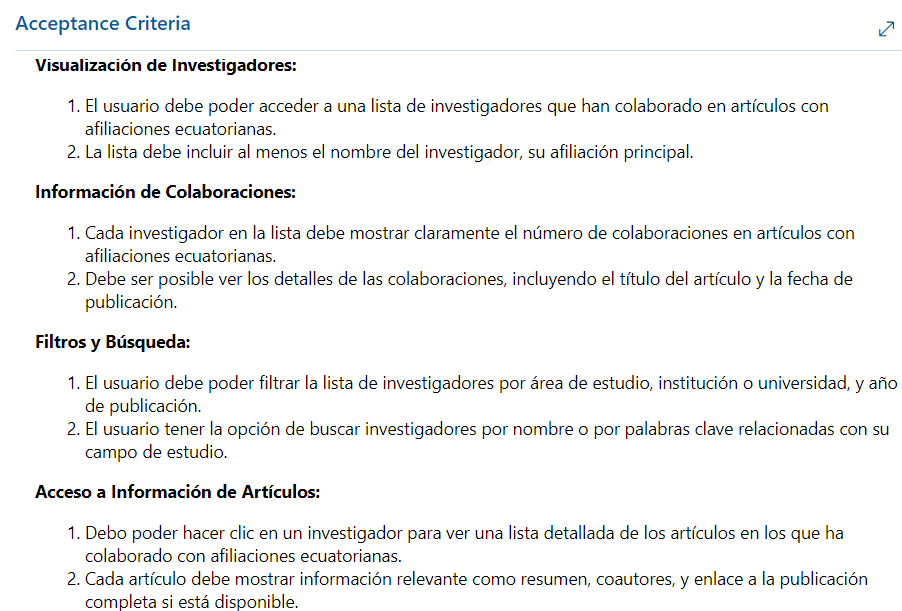
\includegraphics[scale=0.7]{../02Figures/02Chapter/Sprints/Sprint-1/aceptance-criteria-HU-SE-01.png}
    \caption{Criterios de aceptación de las historias de usuario HU-SE-01}
    \label{fig:aceptance-criteria-HU-SE-01}
\end{figure}
\begin{figure}[H]
    \centering
    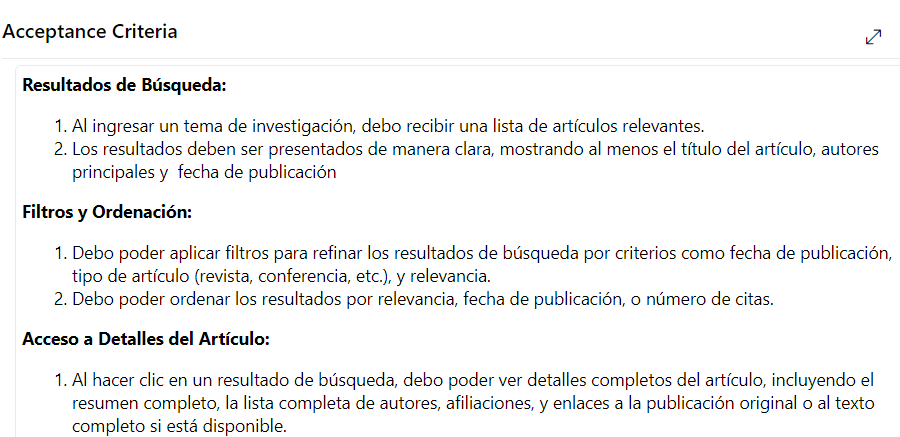
\includegraphics[scale=0.7]{../02Figures/02Chapter/Sprints/Sprint-1/aceptance-criteria-HU-SE-02.png}
    \caption{Criterios de aceptación de la historia de usuario HU-SE-02}
    \label{fig:aceptance-criteria-HU-SE-02}
\end{figure}


Estas historias de usuario se han priorizado en función de su importancia y complejidad, y se han asignado a los miembros del equipo de desarrollo. La figura \ref{fig:azure-board-sprint-1} muestra las tareas asignadas a cada miembro del equipo.
\begin{figure}[H]
    \centering
    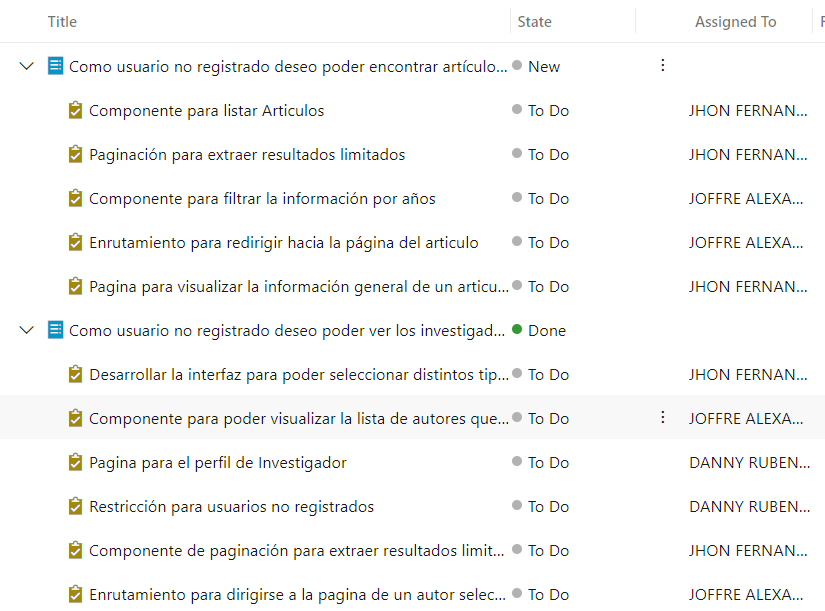
\includegraphics[scale=0.9]{../02Figures/02Chapter/Sprints/Sprint-1/fig_azure-board-sprint-1.png}
    \caption{Planificación de tareas del Sprint 1}
    \label{fig:azure-board-sprint-1}
\end{figure}

\subsection{Implementación}
Para la implementación de las historias de usuario, se ha utilizado la herramienta de diseño Figma, que permite crear prototipos de alta y baja fidelidad. 
A continuación, se presentan los mockups de las interfaces de usuario de la aplicación que se han desarrollado durante este sprint.
Cabe destacar que se siguio un proceso iterativo, por lo que los mockups presentados no son definitivos y pueden sufrir cambios en futuras iteraciones.
Ademas el diseño se baso en el patron de diseño Mobile First, que consiste en diseñar primero la versión móvil de la aplicación y luego adaptarla a dispositivos de mayor tamaño.

\subsubsection{Página de inicio}
La página de inicio de la aplicación es la primera pantalla que verá el usuario al ingresar a la plataforma. 
En esta pantalla, se mostrarán las opciones de búsqueda y un conjunto de datos sobre la información que tiene Centinela. Así como también una barra de navegación que permitirá al usuario acceder a otras secciones de la aplicación. 
La figura \ref{fig:mockup-home} muestra el diseño de la página de inicio.

\begin{figure}[H]
    \centering
    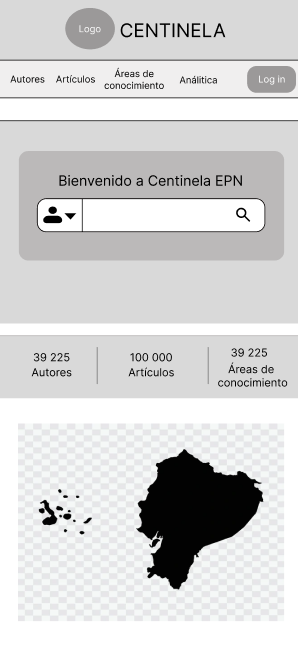
\includegraphics[scale=0.9]{../02Figures/02Chapter/Sprints/Sprint-1/mobile-first-home.png}
    \caption{Mockup de la página de inicio}
    \label{fig:mockup-home}
\end{figure}

Como se menciono en la sección \ref{chapter02-section02-sprint0} se utilizara una adaptación de arquitectura hexagonal para desarrollar la estructura de la aplicación.
Dando como resultado la estructura de carpetas que se muestra en la figura \ref{fig:hexagonal-architecture-home}.
Puesto que la página de inicio es la primera pantalla que verá el usuario al ingresar a la plataforma, se ha decidido crear una carpeta específica para esta sección.
Tambien debido a que angular es un framework que se maneja con componentes, se ha creado un componente para la página de inicio, el cual se encuentra en la carpeta de pages.
A su vez  se ha creado el archivo de tipo module para la página de inicio, el mismo nos permitira importar los componentes necesarios para la página de inicio, sin tener que importarlos en el archivo principal de la aplicación.
Este enfoque permitira que el modulo de la página de inicio sea independiente del resto de la aplicación, que juntado con la arquitectura hexagonal facilitara la escalabilidad y mantenimiento de la aplicación.

\begin{figure}[H]
    \centering
    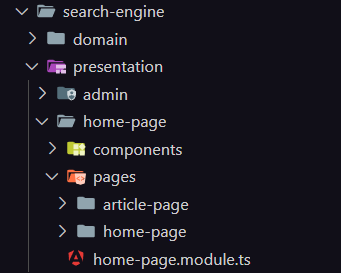
\includegraphics[scale=0.8]{../02Figures/02Chapter/Sprints/Sprint-1/home-page-ha.png}
    \caption{Estructura de carpetas de la página de inicio}
    \label{fig:hexagonal-architecture-home}
\end{figure}

Resultado de la implementación de la página de inicio se muestra en la figura \ref{fig:home-page}.
En la que se muestra la barra de navegación, el formulario de búsqueda y la información que tiene Centinela. El formulario de búsqueda cuenta con 3 opciones, 
la primera es para buscar por palabra clave a un autor, la segunda es para buscar autores relevantes dado un tópico de investigación y la tercera es para buscar articulos relevantes dado un tópico.
Bajo el motor de busqueda se muestra el resumen del numero de articulos, autores y topicos que tiene registrado Centinela.
Finalmente contiene un mapa que mostrará en que el número de articulos que se han publicado en cada provincia del Ecuador.
\begin{figure}[H]
    \centering
    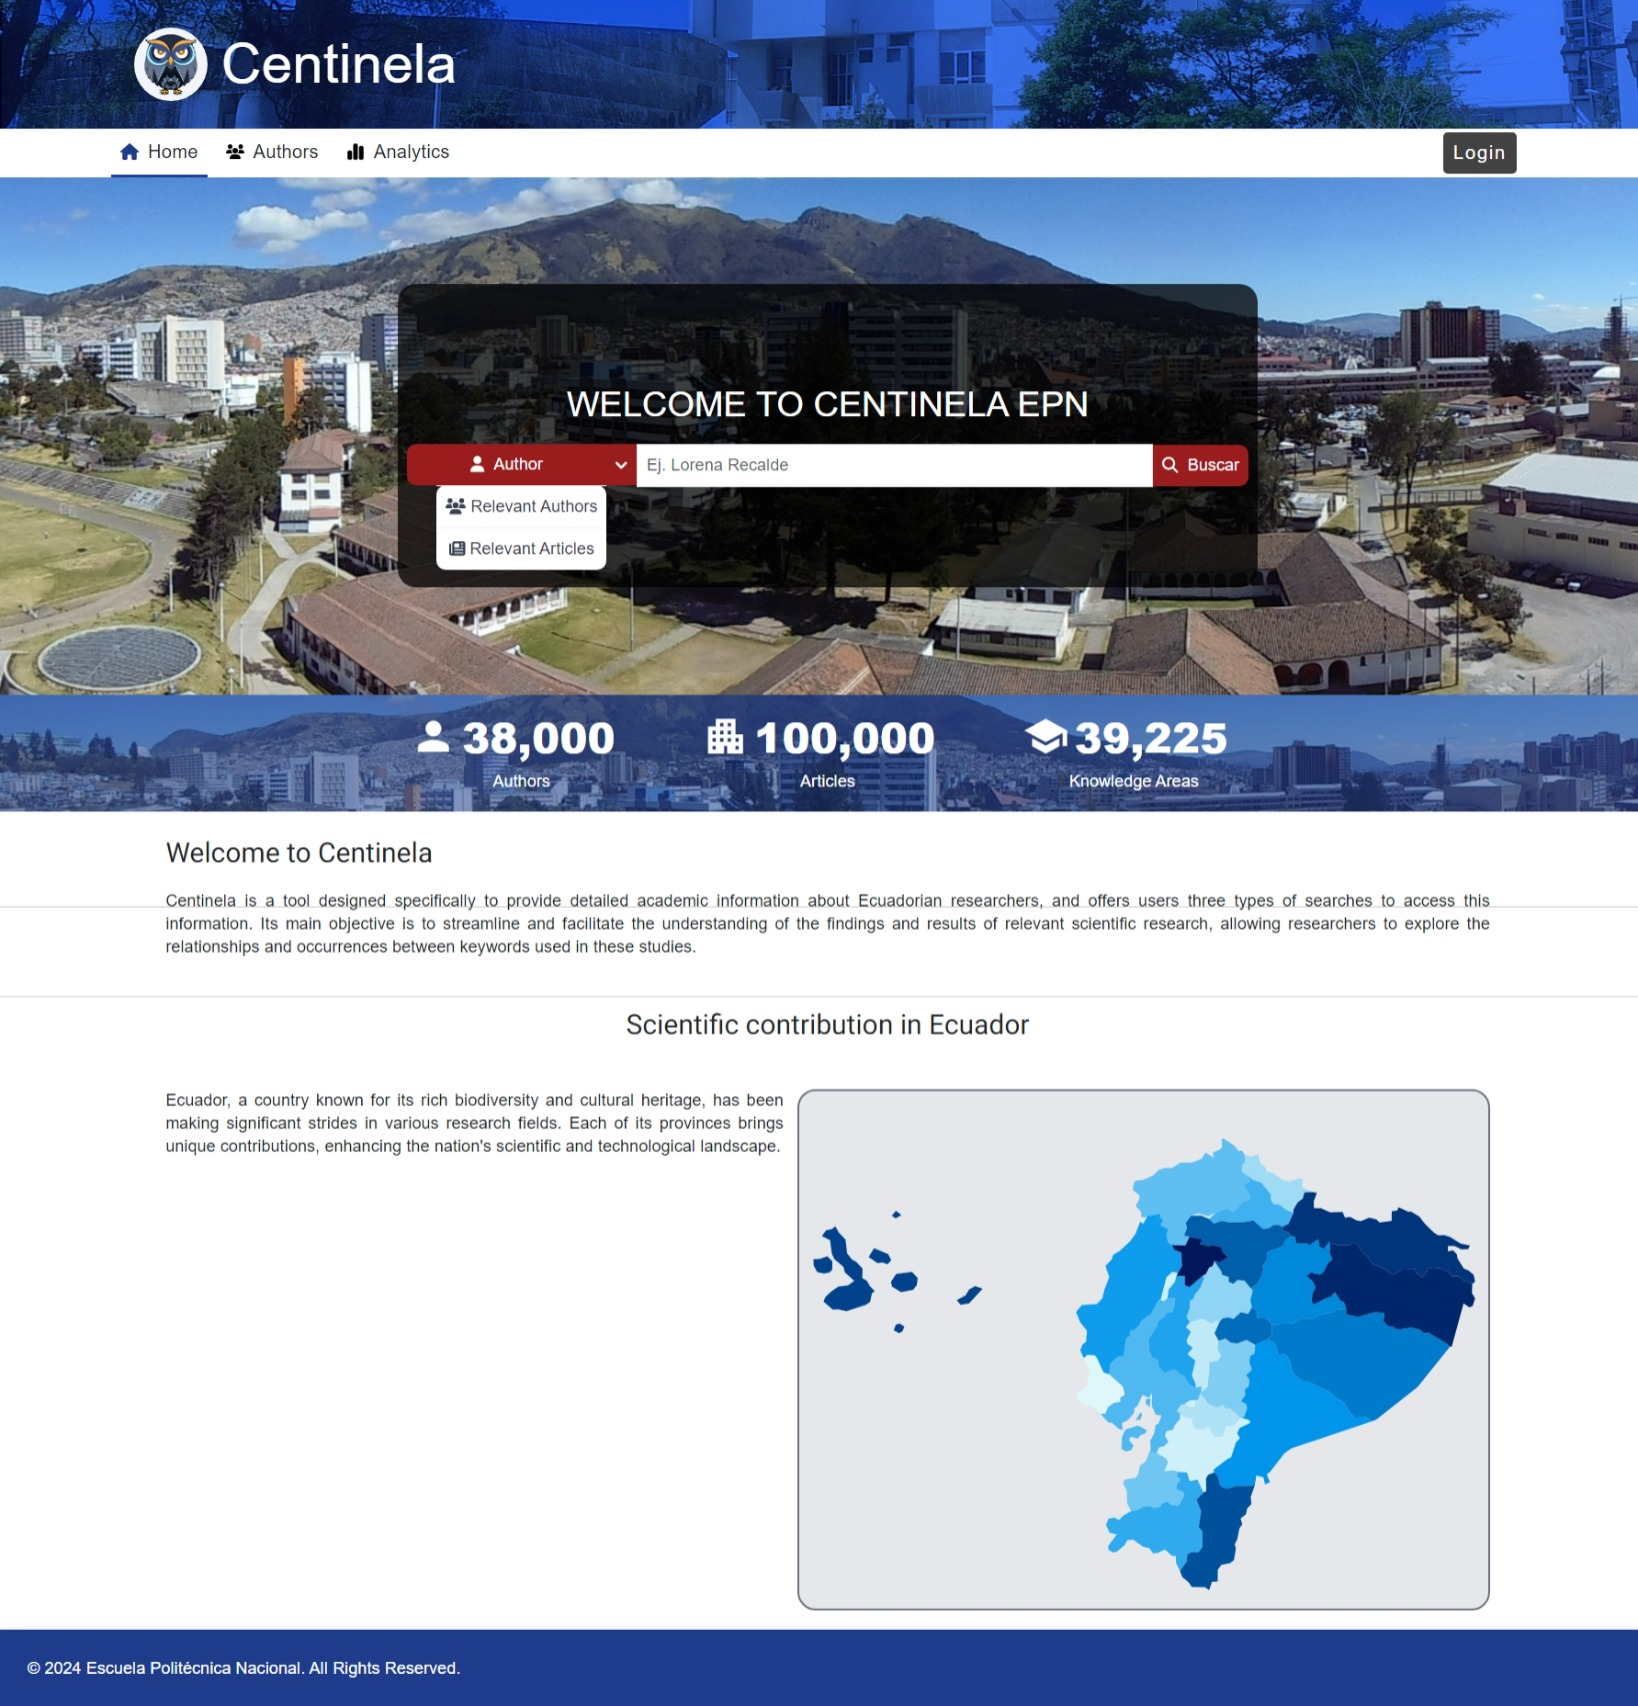
\includegraphics[scale=0.160]{../02Figures/02Chapter/Sprints/Sprint-1/home-page.jpeg}
    \caption{Página de inicio}
    \label{fig:home-page}
\end{figure}

\subsubsection{Página de resultados}
La página de resultados es la pantalla que se mostrará al usuario después de realizar una búsqueda en la aplicación.
En esta pantalla, se mostrarán los resultados de la búsqueda, que incluirán una lista de autores y artículos relevantes, dependiendo del tipo de búsqueda que haya realizado el usuario.
La figura \ref{fig:mockup-results} muestra el diseño de la página de resultados. Cabe destacar que esta página va a ser dinamica, es decir se modificará en función de los resultados de la búsqueda.
También contiene el componente de paginación, que permitirá al usuario navegar entre los resultados de la búsqueda. Este último está disponible para el tipo de busqueda de autores por palabra clave y para el tipo de busqueda de articulos relevantes por tópico, ya que estos tipos de busqueda pueden devolver un gran número de resultados. Y al ser una aplicación web, se ha optado por mostrar 10 resultados por página para garantizar una buena experiencia de usuario y reducir tiempos de carga.

\begin{figure}[H]
    \centering
    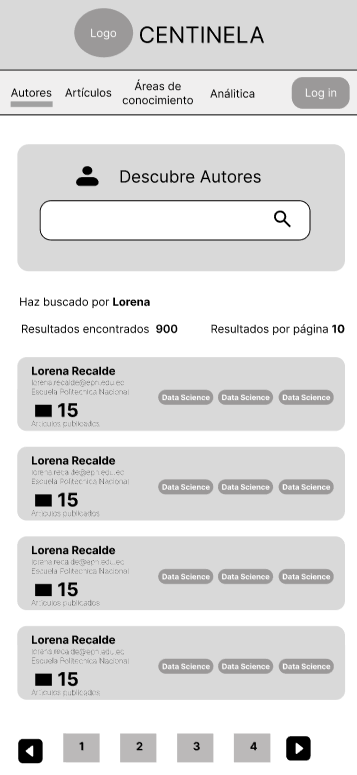
\includegraphics[scale=0.6]{../02Figures/02Chapter/Sprints/Sprint-1/mobile-first-results.png}
    \caption{Mockup de la página de resultados}
    \label{fig:mockup-results}
\end{figure}

Como se menciono en la Tabla \ref{fig:aceptance-criteria-HU-SE-01} y \ref{fig:aceptance-criteria-HU-SE-02} los criterios de aceptación de las historias de usuario HU-SE-01 y HU-SE-02 cada resultado tendra que ser redirigido a una pantalla en donde 
se visualizará la información detallada del autor o del articulo. Para este caso en especifico se muestra el diseño para la pagina que tendra
la información detallada de un autor, en la figura \ref{fig:mockup-article-detail}.
\begin{figure}[H]
    \centering
    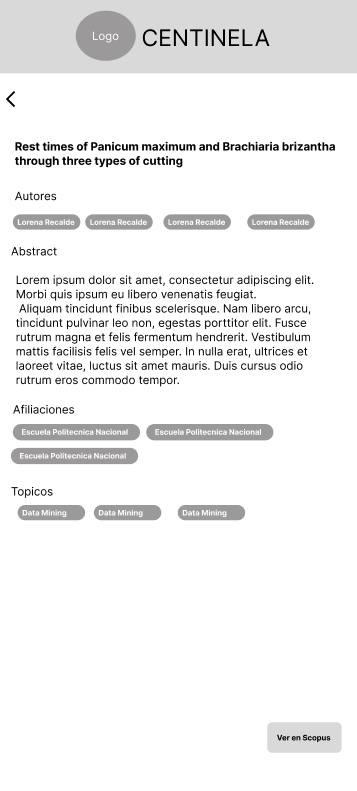
\includegraphics[scale=0.8]{../02Figures/02Chapter/Sprints/Sprint-1/article-detail.png}
    \caption{Mockup de la página de detalle de autor}
    \label{fig:mockup-article-detail}
\end{figure}

Para el enrutamiento de la aplicación se ha utilizado el modulo de enrutamiento de Angular, el cual nos permite definir las rutas de la aplicación y asociarlas con los componentes correspondientes.
En la Figura \ref{fig:enrutamiento-article-page} se muestra el enrutamiento hacia el componente que contendra la información general de un articulo. El mismo que como parametro recibirá el id del articulo que se desea visualizar.
\begin{figure}[H]
    \centering
    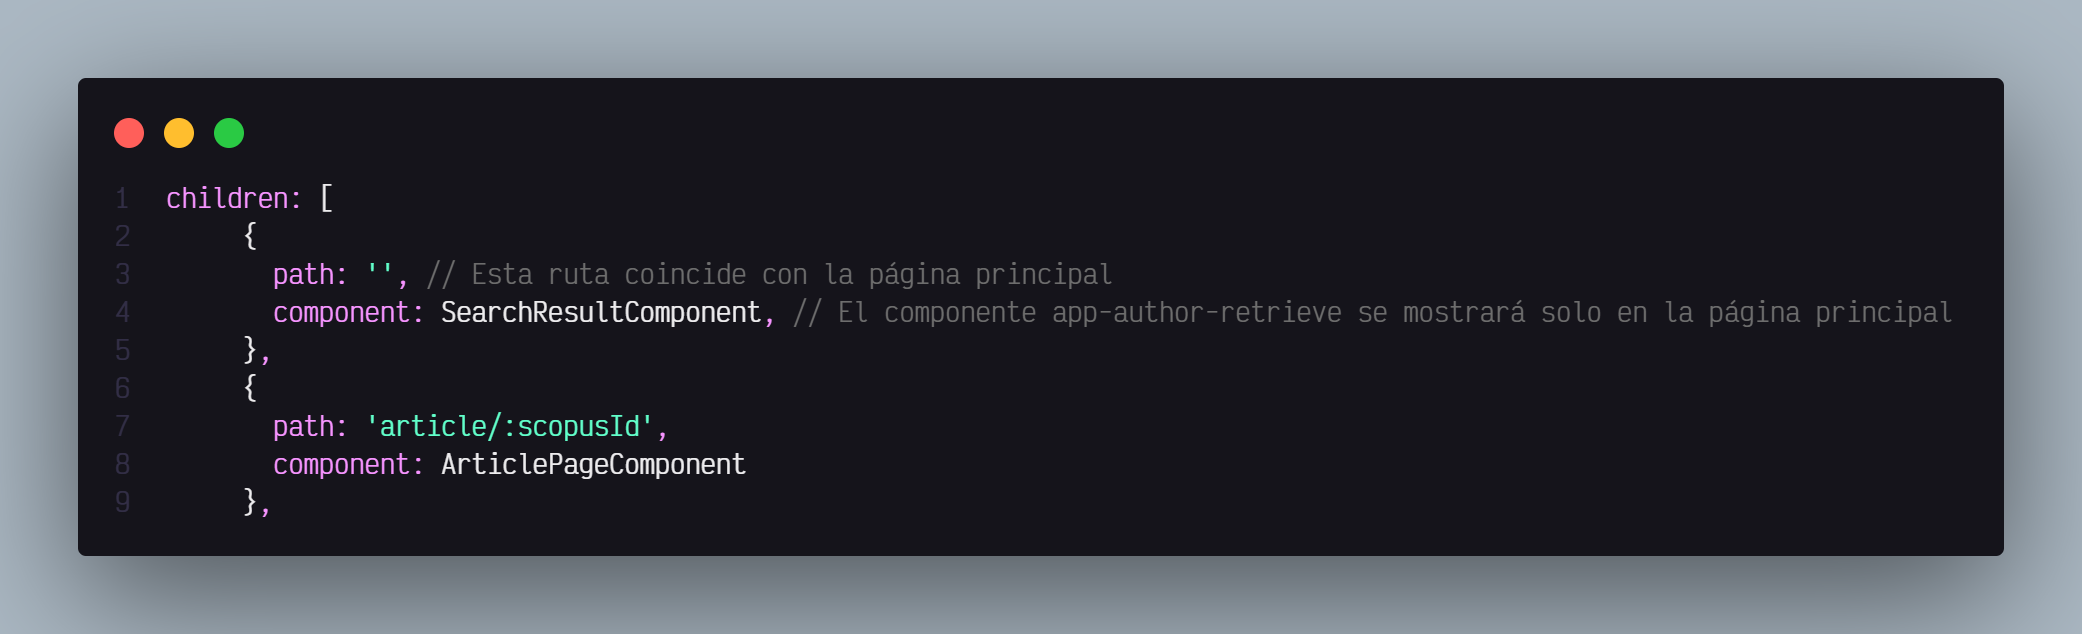
\includegraphics[scale=0.2]{../02Figures/02Chapter/Sprints/Sprint-1/enrutamiento-article-page.png}
    \caption{Routing de la página de detalle de articulo}
    \label{fig:enrutamiento-article-page}
\end{figure}

%% Aqui deseo mostrar ya la implementacion de la pagina de articulo pero da una descripcion de la misma
Resultado de la implementación de la página de información general de un articulo se muestra en la figura \ref{fig:article-page}.
En la que se muestra la información general de un articulo, como el titulo, resumen, autores, afiliaciones, palabras clave y el año de publicación. Asi como tambien un boton que permitira al usuario acceder al articulo completo en la pagina de Scopus.

\begin{figure}[H]
    \centering
    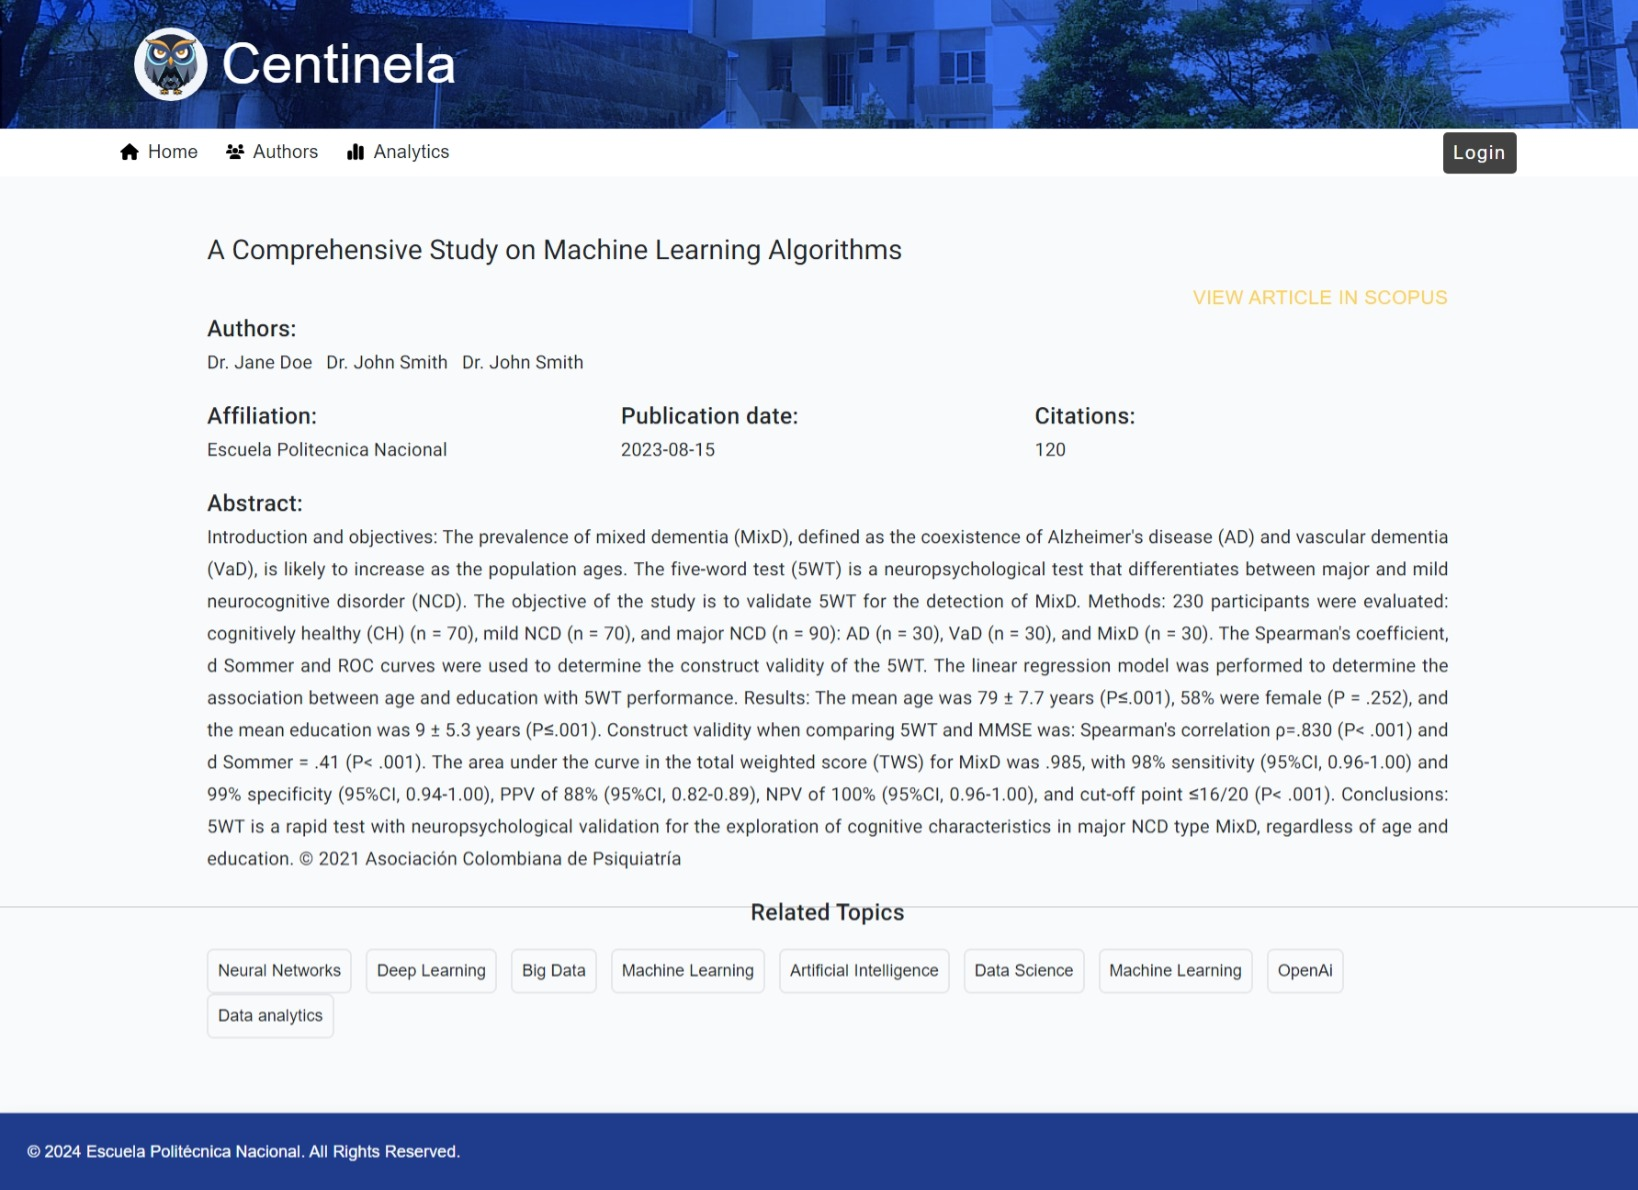
\includegraphics[scale=0.160]{../02Figures/02Chapter/Sprints/Sprint-1/article-page.jpeg}
    \caption{Página de detalle de articulo}
    \label{fig:article-page}
\end{figure}

%% Revision y Retrospectiva del sprint
\subsection{Revisión y Retrospectiva del Sprint}
Durante este sprint, hemos logrado completar todas las historias de usuario planificadas, lo que nos ha permitido avanzar significativamente en el desarrollo de la aplicación.
Hemos creado los mockups de las interfaces de usuario de la aplicación, desarrollado la estructura principal del motor de búsqueda, implementado el enrutamiento de la aplicación y la página de inicio.
Además, hemos implementado la página de resultados y la página de información general de un artículo.
En general, el equipo ha trabajado de manera eficiente y colaborativa, lo que ha permitido cumplir con los objetivos del sprint en el tiempo previsto.
Sin embargo, hemos identificado algunas áreas de mejora que podrían ayudarnos a optimizar nuestro trabajo en futuros sprints.
\begin{itemize}
    \item \textbf{Comunicación}: Aunque hemos mantenido una comunicación constante a través de reuniones diarias y canales de mensajería, es importante mejorar la comunicación entre los miembros del equipo para garantizar que todos estén al tanto de los avances del proyecto.
    \item \textbf{Planificación}: Aunque hemos logrado completar todas las historias de usuario planificadas, es importante revisar y ajustar nuestra planificación para futuros sprints, teniendo en cuenta la complejidad y el tiempo requerido para cada tarea.
    \item \textbf{Colaboración}: Hemos trabajado de manera colaborativa y eficiente durante este sprint, lo que ha permitido cumplir con los objetivos del proyecto. Es importante seguir fomentando la colaboración entre los miembros del equipo para garantizar el éxito del proyecto.
    \item \textbf{Retroalimentación}: Es importante recopilar y analizar la retroalimentación de los usuarios para identificar áreas de mejora y realizar ajustes en futuras iteraciones del proyecto.
\end{itemize}